\section{سوال ششم}

در تمرین قبلی با مفهوم فایل سیستم‌ها در لینوکس آشنا شدیم.

برای بررسی فایل سیستم \texttt{proc} می‌توانید از توضیحات موجود در دستور \texttt{man} استفاده کنید:

\begin{latin}
	\texttt{\$ man proc}
\end{latin}

در دایرکتوری هر پردازه در فایل‌سیستم Proc یک فایل به‌نام maps وجود دارد که اطلاعات مربوط به map memory هر پردازه را در آن نگه می‌دارد. \\ \\


\textbf{امتیازی: }با استفاده از \texttt{proc man} یکی از این فایل‌ها را مثلا
\begin{latin}
	\texttt{proc/1/maps}
\end{latin}
را بررسی کنید و هر یک از ستون‌های آن را توضیح دهید که چه چیزی را نمایش می‌دهد.


\begin{qsolve}
با دستور زیر فایل \texttt{maps} یکی از PID های دلخواه‌مان را باز می‌کنیم:

\begin{latin}
	\texttt{\$ sudo vim /proc/1/maps} 
\end{latin}

خروجی فایل به صورت زیر است:
\begin{center}
	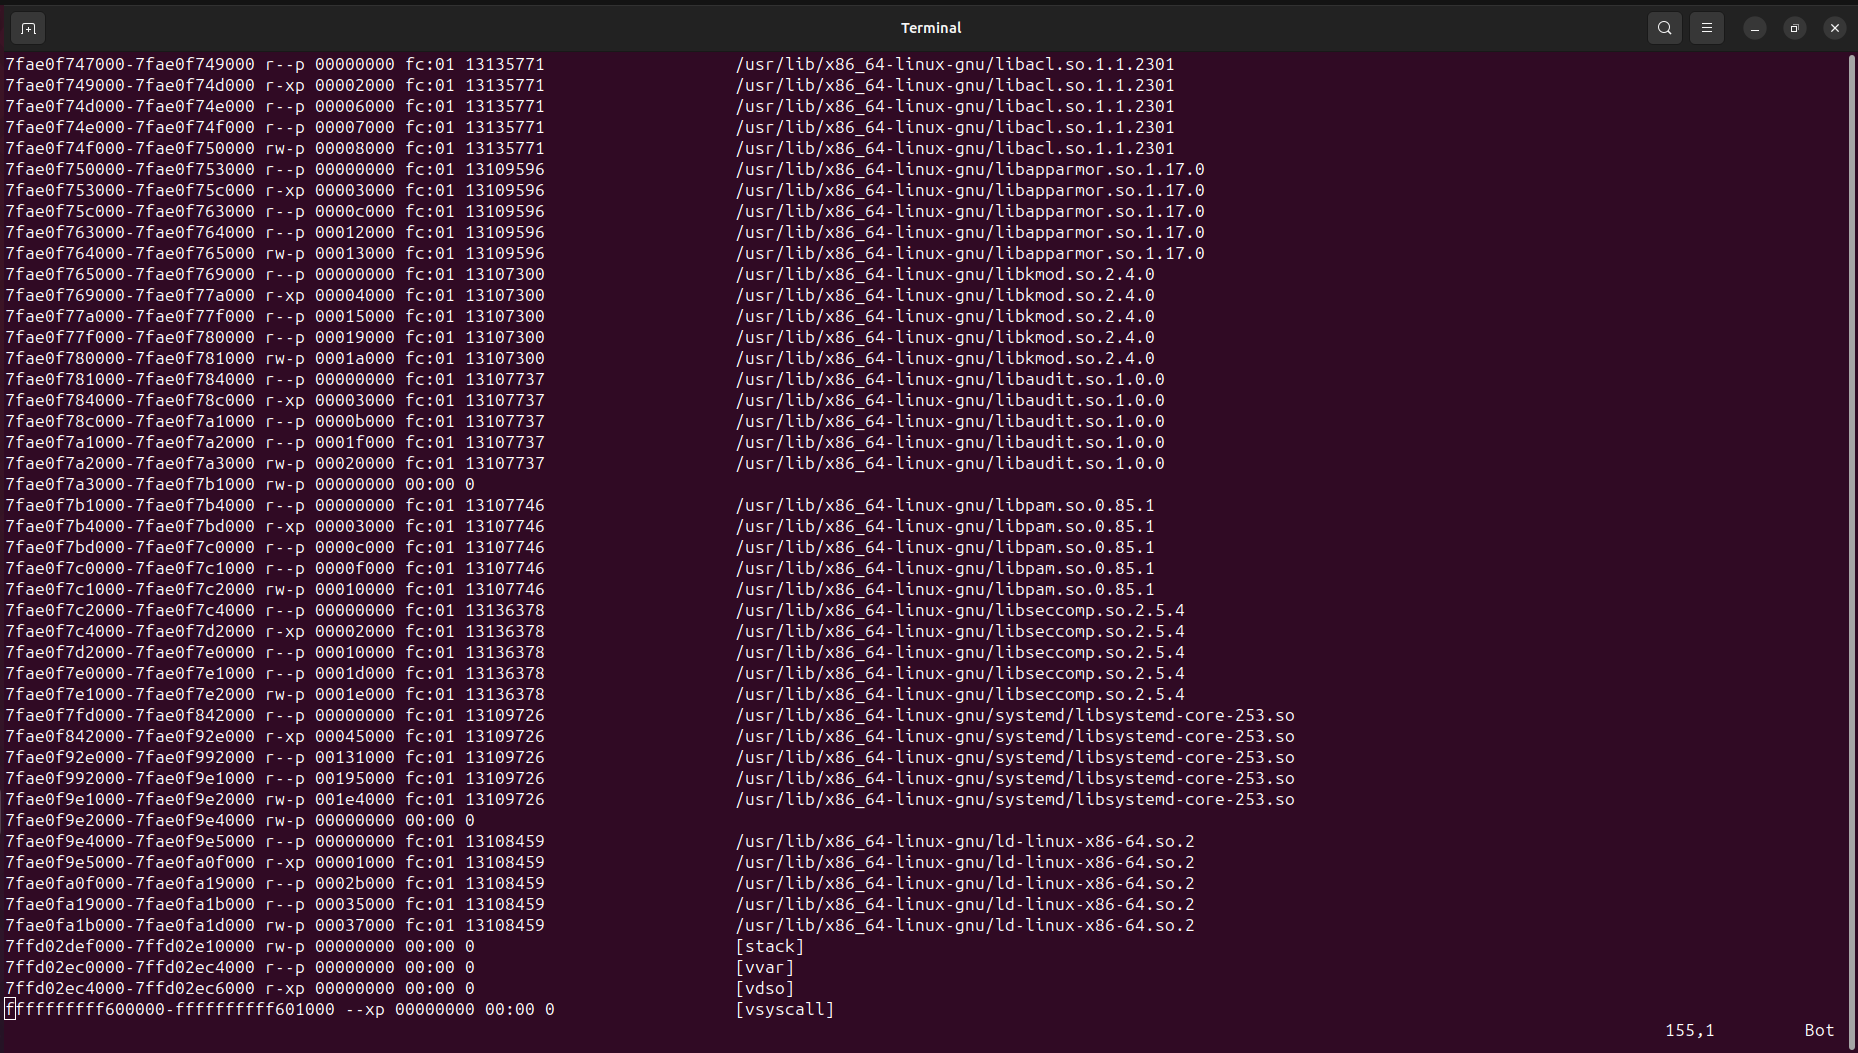
\includegraphics[width=\textwidth]{pics/img1.png}
\end{center}

ساختار هر خط به صورت زیر است:

\begin{enumerate}
	\item \textbf{آدرس شروع-آدرس پایان:}
	نمایانگر محدوده آدرس حافظه است که این ناحیه در آن قرار دارد. آدرس شروع نشان‌دهنده ابتدای ناحیه و آدرس پایان نشان‌دهنده انتهای آن است.
	\item \textbf{دسترسی‌ها:}
	نشان‌دهنده میزان دسترسی‌ها به حافظه است. به عنوان مثال، \texttt{r-x} نشان‌دهنده دسترسی خواندن و اجرا (ولی نه نوشتن) به حافظه است.
	
	\item \textbf{آفست:}
	نشان‌دهنده offset نسبت به نقطه شروع فایل (اگر موجود باشد) یا offset نسبت به ابتدای ناحیه حافظه است.
	
	\item \textbf{دسته حافظه:}
	نشان‌دهنده نوع حافظه استفاده شده، مثل stack, heap و ... است.
	
	\item \textbf{حقوق:}
	نشان‌دهنده حقوق دسترسی به فایل یا ناحیه حافظه است.
	
	\item \textbf{دستگاه :minumum}
	در صورتی که ناحیه حافظه minumum باشد، این ستون نشان‌دهنده number minor دستگاهی است که minumum به آن متصل شده است.
	
	\item \textbf{شماره :minumum}
	
	
	\item \textbf{فایلی که متعلق به حافظه است:}
	اگر ناحیه حافظه به یک فایل متصل باشد، این ستون نشان‌دهنده مسیر فایل است. 
\end{enumerate}

\end{qsolve}